\chapter{Richards flow -- H-Processes}
\label{sec:Richards}
\section{Theory}
\subsection{Single continuum}
Richards equations are used to describe water movement in
unsaturated zone, which is the portion of the subsurface above the
ground water table. Pressure $p$ based formation, that select the
unknown primary variable as $p$, is solved.\\
\begin{eqnarray}\label{eqn:pbased}
n\frac{\partial S^l}{\partial p^l}\frac{\partial p^l}{\partial
t}-\bigtriangledown\cdot\bigg(-\frac{\PermRelP
^l\mathbf{k}}{\mu^l}(\bigtriangledown
p^l-\rho^l\mathbf{g})\bigg)=\frac{Q_{\rho^l}} {\rho^l}
\end{eqnarray}\\

Constitutive equations are described as:
\begin{description}
  \item[Saturation:]
    \begin{eqnarray}
    \theta = n S
    \end{eqnarray}
    \begin{eqnarray}
     \SaturationEff=\frac{S-S_r}{\SaturationMax-\SaturationRes}
    \end{eqnarray}
  \item[Pressure:]
    \begin{eqnarray}
    p_c = -p^l
    \end{eqnarray}
    van Genuchten model
    \begin{eqnarray}
    p_c = \frac{\rho g}{\alpha}(\SaturationEff^{-1/m}-1)^{1/n}
    \end{eqnarray}
    \begin{eqnarray}
    m=1-\frac{1}{n}
    \end{eqnarray}
  \item[Permeability:] Relationship of hydraulic conductivity and
  permeability:
    \begin{eqnarray}
    \mathbf{k}=\frac{\mu}{\rho g}\mathbf{K}
    \end{eqnarray}
    van Genuchten model [van Genuchten, 1980]
    \begin{eqnarray}
    \PermRelP &=& \SaturationEff^{1/2} \left[
            1-(1-\SaturationEff^{1/m})^m \right]^2
    \end{eqnarray}
\end{description}

Tangent approximation is applied for capacity coefficient
$M=\frac{\partial S^l}{\partial p^l}$, and combined with
mass-lumping matrix to reduce oscillation and improve numerical
stability. Picard iteration scheme is used for nonlinear iterations. \\

\subsection{Dual continua}
In structured porous media the water movement can be described by
dual-porosity model, which is composed by coupled Richards
equations of matrix and fracture continua, respectively, which are
combined by additional transfer and specific storage terms.\\
\begin{eqnarray}\label{eqn:pbased_m}
n\frac{\partial S^l_m}{\partial p^l_m}\frac{\partial
p^l_m}{\partial t}-\bigtriangledown\cdot\bigg(\frac{\PermRelP
^l\mathbf{k}_m}{\mu^l}(\bigtriangledown
p^l_m-\rho^l\mathbf{g})\bigg)=\frac{Q_{\rho^lm}}
{\rho^l}+\frac{\Gamma^l}{w_m}
\end{eqnarray}
\begin{eqnarray}\label{eqn:pbased_f}
n\frac{\partial S^l_f}{\partial p^l_f}\frac{\partial
p^l_f}{\partial t}-\bigtriangledown\cdot\bigg(\frac{\PermRelP
^l\mathbf{k}_f}{\mu^l}(\bigtriangledown
p^l_f-\rho^l\mathbf{g})\bigg)=\frac{Q_{\rho^lf}}
{\rho^l}-\frac{\Gamma^l}{w_f}
\end{eqnarray}
Relationship of preferential factors $w_m$ and $w_f$ is:
\begin{eqnarray}
w_m+w_f = 1
\end{eqnarray}
Transfer term is given as follows:
\begin{eqnarray}\label{eqn:pbased}
\Gamma^l =\alpha^\ast K_{\alpha}(p^l_f-p^l_m)R^l
\end{eqnarray}
The first-order exchange coefficient $\alpha^\ast$ [1/s] is
derived from the properties of the fractures network, which also
define the average size and form of the matrix blocks as $A^\ast
\beta/D$, where $A^\ast$ is the fracture/matrix interface area per
bulk volume of rock [$m^3/m^3$], $\beta$ is a shape factor, and D
is the average fracture spacing [m](or average matrix block size).
$K_{\alpha}$ is the hydraulic conductivity at the interface
between fracture and matrix continua, usually define $K_{\alpha}$
as the unsaturated hydraulic conductivity of the matrix rock,
because the much smaller matrix permeability is the limiting
factor for fracture-matrix flow. Interface reduction factor $R^l$
is set to the fracture liquid saturation $S^l_f$. The saturation
of whole system is:
\begin{eqnarray}
S=S_mw_m+S_fw_f
\end{eqnarray}\\
\subsubsection{Numerical methods}
There are two numerical methods used to solve dual-continua model:
partitioned and monothlic, which are given as the following
descriptions.
\subsubsection*{Partitioned}
In the partitioned scheme, two coupled Richards equations are
solved one after another: one primary variable is given as known
value when the other is solved, and the system error is controlled
by the first primary variable.
%\begin{eqnarray}\label{eqn:mono-m-c}
%[A_{mij}]\{dp_{mi}/dt\}+[B_{mij}]\{p_{mi}\}=\{F_{mi}\}
%\end{eqnarray}
%\begin{eqnarray}\label{eqn:mono-f-c}
%[A_{fij}]\{dp_{fi}/dt\}+[B_{fij}]\{p_{fi}\}=\{F_{fi}\}
%\end{eqnarray}
%----------------------------------------
\subsubsection*{Monolithic}
All the primary variables are assembled in one matrix and solved
as unknown variables in the same time in monolithic scheme.
%\begin{eqnarray}\label{eqn:mono-m}
%[A_{mij}]\{dp_{mi}/dt\}+[B_{mij}]\{p_{mi}\}-[C_{mij}]\{p_{fi}\}=\{F_{mi}\}
%\end{eqnarray}
%\begin{eqnarray}\label{eqn:mono-f}
%[A_{fij}]\{dp_{fi}/dt\}+[B_{fij}]\{p_{fi}\}-[C_{fij}]\{p_{mi}\}=\{F_{fi}\}
%\end{eqnarray}

%\newpage

\section{Single Continuum}
%
Single continuum model is based on Eq. \ref{eqn:pbased}.
%
\subsection{Infiltration in homogenous soil}
\label{sec:Warrick}
\subsubsection*{Problem definition}
This case is a numerical modelling of classical experiment of
Warrick et al's(1971)\cite{Warrick:1971}. The solution is Richards
equation combining with uniform initial condition, fixed boundary
condition without source term, and curve descriptions of
homogenous media properties.\\
As for the dimension extension, line, triangle, quadrilteral, hexahedra, prism and tetrahedra mesh are used, and distinctions of different special discretization are presented in right of Fig. \ref{us:warrick}. Here, we present temporal evolution of the capillary pressure at the some point.
%
\subsubsection*{Initial and boundary conditions}
The uniform initial condition in the whole domain, the saturation
is 0.455, and meanwhile the pressure is -21500 Pa. Boundary
condition at the top is saturated, accordingly pressure is 0, and
pressure equals -21500 Pa at bottom in the simulation period.
Details are
illustrated in left of Fig. \ref{us:warrick}.\\
%-------------------------------------------------
\begin{figure}[thbp]
\centerline{\psfig{figure=H_US/figures/illustration_warrick.eps,height=1.75in,width=1.75in}\psfig{figure=H_US/figures/ele_test_warrick.eps,height=1.75in,width=1.75in}}
\caption{Illustration of numerical model and element test.}
\label{us:warrick}
\end{figure}
%-------------------------------------------------
%
\subsubsection*{Material properties}
Homogenous material properties are assumed within the whole
domain. Table \ref{us:warricksetting} gives the parameters.\\
%------------------------------
\begin{table}[H]
 \centering
 \caption{Parameters in simulation}
 \centering \label{us:warricksetting}
 \begin{tabular}{llll}
 \hline\hline\noalign{\smallskip}
 items & setting  \\ \hline
 Porosity              & 0.38 \\
 Capillary pressure    & $p(S)$ Curve in Fig. \ref{us:warrickpks}(l) \\
 Relative permeability & $k_{rel}$Curve in Fig. \ref{us:warrickpks}(r)\\
 Permeability tensor $(m^2)$  &  9.35e-12  \\
\noalign{\smallskip}\hline\hline
 \end{tabular}
\end{table}
%------------------------------
\begin{figure} [htb!]
 \centering 
 \includegraphics[width=0.85\columnwidth] {H_US/figures/warrick-p-k-s.eps}
 \caption{Relationship of capillary pressure-saturation and relative permeability-saturation}
 \label{us:warrickpks}
\end{figure}
%------------------------------
\subsubsection*{Results}
Fig. \ref{us:result-warrick} shows the distribution of saturation.
Symbols in the Fig.\ref{us:result-warrick} are observations of
Warrick et al's(1971)\cite{Warrick:1971}.

\begin{figure} [!htb]
 \centering
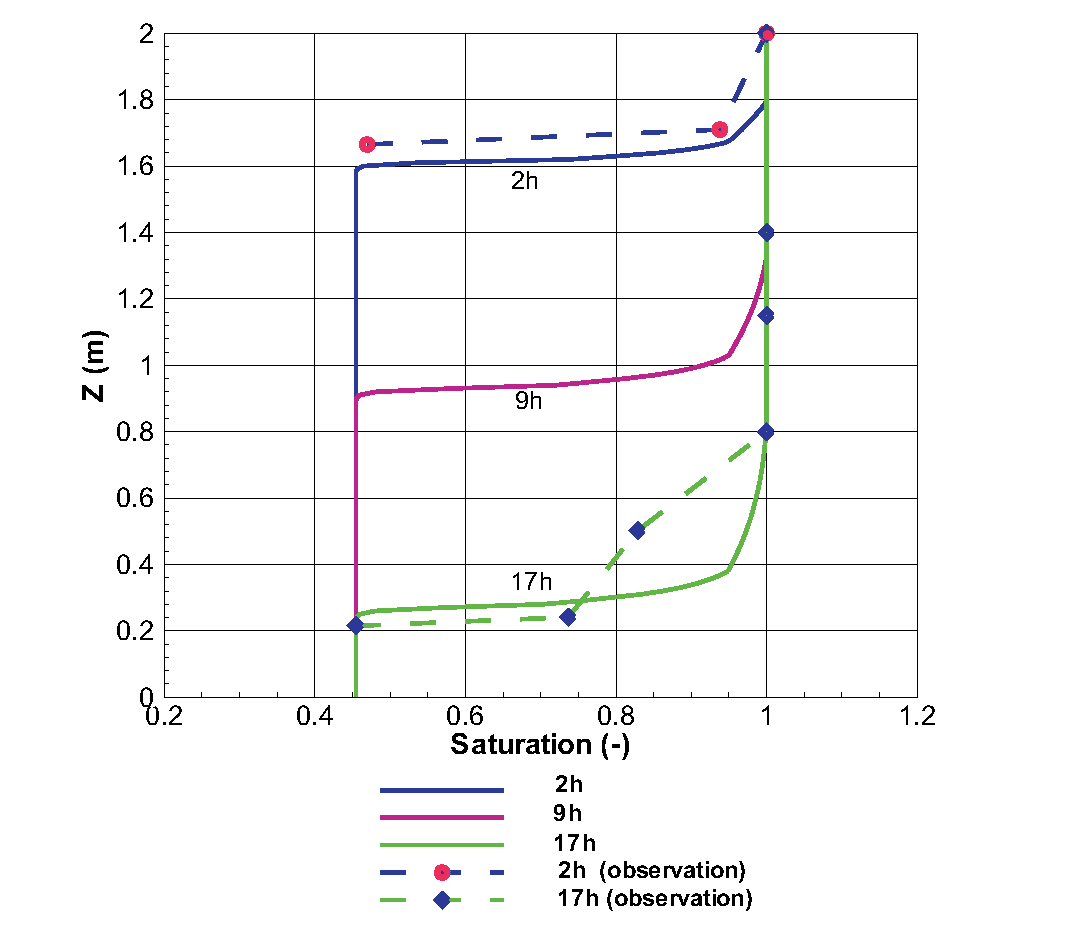
\includegraphics[width=0.6\columnwidth]{H_US/figures/result_warrick.eps}
\caption{Saturation comparison of observed (symbol and dashed) and
simulated (solid)} \label{us:result-warrick}
\end{figure}

%-------------------------------------------------
%
Fig. \ref{us:result-warrick2D} shows the distribution of
saturation by triangle and quadrilateral mesh respectively, the
symbol-solid lines are 1D results. When the mesh densities are
identical, the results are same; otherwise, there are
distinctions.
% as Fig. \ref{us:result-warrick-comparison}.
%-------------------------------------------------
\begin{figure}[h]
\centering \vspace{2.5cm} \unitlength1cm
\begin{minipage}[t]{5.5cm}
\begin{picture}(5.5,4.5)
\includegraphics[height=1.2\columnwidth, angle=0]{H_US/figures/result_warrick_tri.eps}
\end{picture}\par
\end{minipage}
\hfill
\begin{minipage}[t]{5.5cm}
\unitlength1cm
\begin{picture}(5.5,4.5)
\includegraphics[height=1.2\columnwidth, angle=0]{H_US/figures/result_warrick_quad.eps}
\end{picture}
\end{minipage}
%\begin{center}
%\hspace{0.0cm} (a) \hspace{6.0cm} (b)
%\end{center}
\caption{Saturation simulation by triangle(l) and quadrilateral
(r) mesh comparison with 1D mesh (symbol-solid)}
\label{us:result-warrick2D}
\end{figure}
%-------------------------------------------------
%-------------------------------------------------
%\begin{figure} [!htb]
%\centering \vspace{1.1cm} \unitlength1cm
%\begin{minipage}[t]{5.8cm}
%\unitlength1cm
%\begin{picture}(5.8, 4.4)
%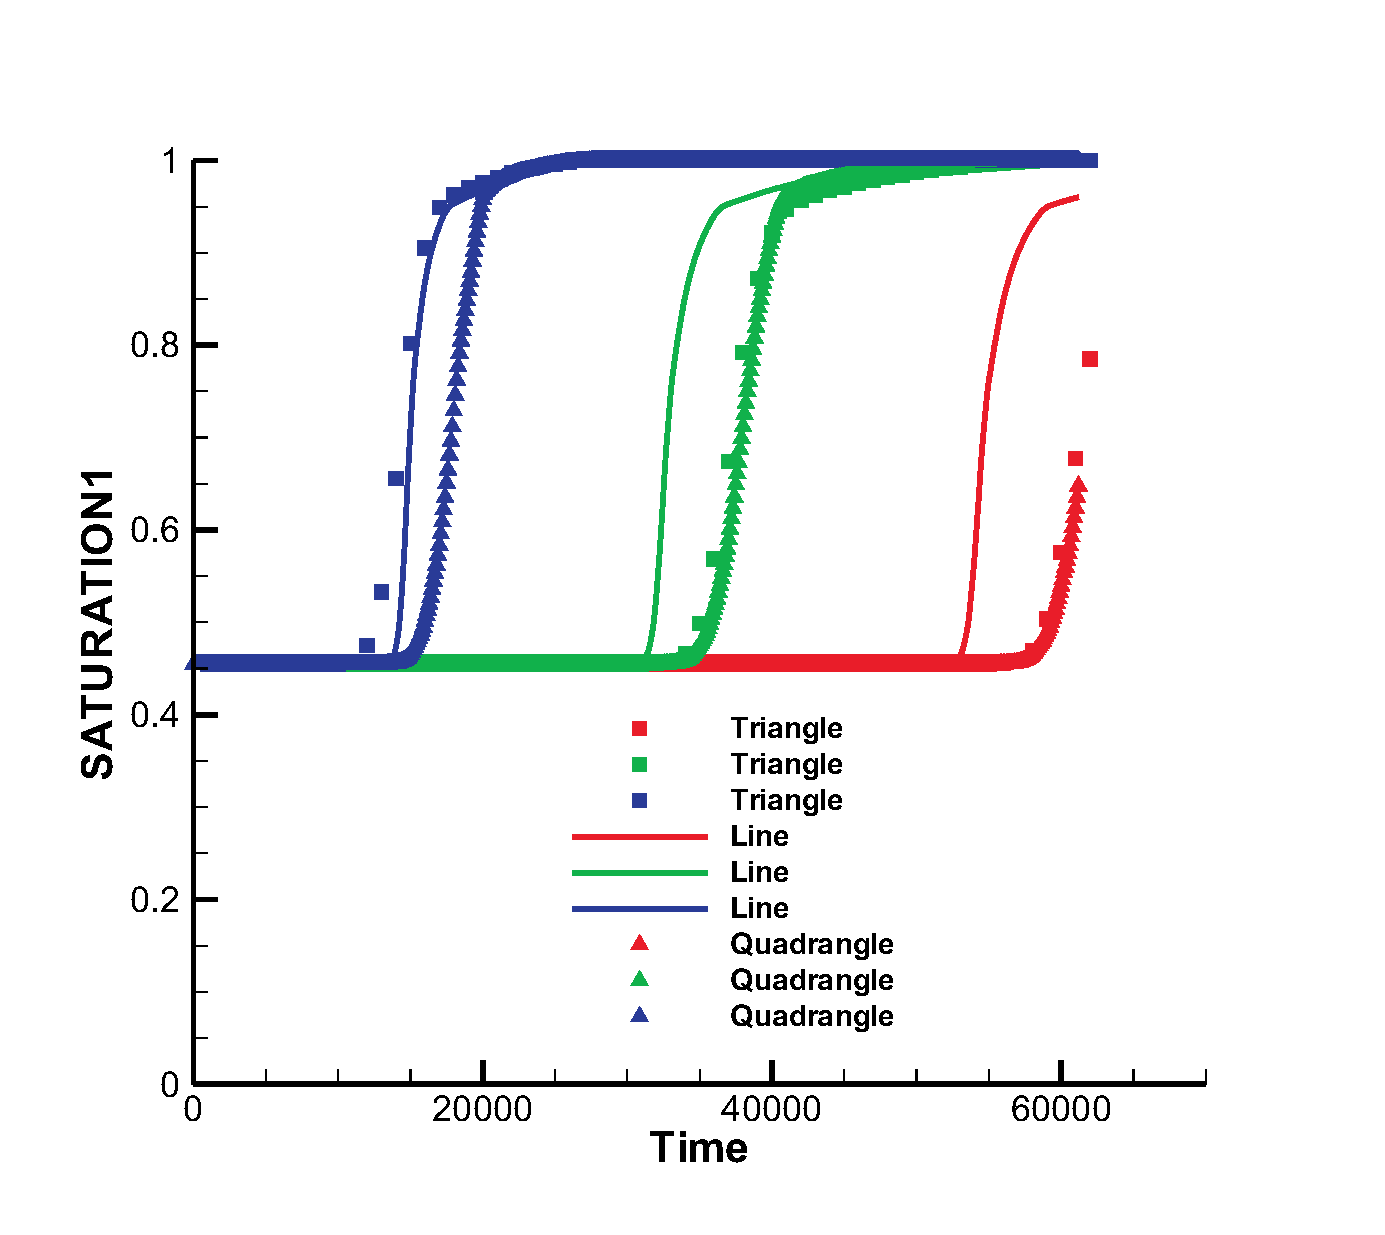
\includegraphics[height=1.05\columnwidth,
%angle=0]{H_US/figures/result_warrick_comparison.eps}
%\end{picture}
%\end{minipage}
%\caption{Comparisons of time evolution of saturation by line,
%triangle and quadrangle mesh}
%\label{us:result-warrick-comparison}
%\end{figure}
%-------------------------------------------------
%------------------------------
\subsubsection*{Benchmark deposit}
\begin{tabular}{|l|l|l|}
  \hline
  Benchmark & Problem type & Path in benchmark deposit \\
  \hline
 \emph{h\_us\_line\_warrick} & H & benchmarks\verb \h_us\wet\ \\
  \hline
  \emph{h\_us\_quad} & H & benchmarks\verb \h_us\wet\ \\
  \hline
  \emph{h\_us\_tri\_freebc} & H & benchmarks\verb \h_us\wet\ \\
  \hline
\end{tabular}

%\newpage

\subsection{Infiltration in homogenous soil (ST/BC)}
%
\subsubsection*{Problem definition}
Numerical results compare with experimental measurements of Abeele
et al.(1981). The soil column is 6m long and the diameter is 3m.
The problem is defined as uniform initial condition, continuous
infiltration treated as source term at top, van Genuchten
homogenous material and constant mesh density.
%
\subsubsection*{Initial, boundary conditions and source term}
The initial condition of pressure is -71000pa, and continuous
source term at the top is 2.314e-6m/s. Details are illustrated in
Fig. \ref{us:forsyth}.
%-------------------------------------------------
\begin{figure} [htb!]
 \centering
 \includegraphics[width=0.25\columnwidth] {H_US/figures/illustration_forsyth.eps}
 \caption{Illustration of numerical model}
 \label{us:forsyth}
\end{figure}
%-------------------------------------------------
\subsubsection*{Material properties}
Homogenous material properties are assumed within the whole
domain. Table \ref{us:forsythsetting} gives the parameters.
%------------------------------
\begin{table}[H]
 \centering
 \caption{Parameters in simulation} \centering \label{us:forsythsetting}
 \begin{tabular}{llll}
 \hline\hline\noalign{\smallskip}
 Parameter    & Value  &  Unit  \\ \hline
 Porosity          & 0.33   & -   \\
 Saturated permeability $k_s$ &2.95e-13 & $m^2$ \\
 $S_r^l$           & 0.0    &  - \\
 $S_{max}^l$        & 1.0    &  - \\
 $\alpha$           & 1.43   &  $1/m$ \\
 $n$                & 1.506  &  - \\
\noalign{\smallskip}\hline\hline
 \end{tabular}
\end{table}
%
\subsubsection*{Results}
Fig. \ref{us:result-forsyth} shows the distribution of saturation.
Left side in Fig.\ref{us:result-forsyth} is the result of
reference \cite{Forsyth:1995}.
%-------------------------------------------------
\begin{figure}[h]
\centering \vspace{0cm} \unitlength1cm
\begin{minipage}[t]{6cm}
\begin{picture}(6,5.5)
\includegraphics[height=0.85\columnwidth, angle=0]{H_US/figures/Reference_forsyth.eps}
\end{picture}\par
\end{minipage}
\hfill
\begin{minipage}[t]{6cm}
\unitlength1cm
\begin{picture}(6,5.5)
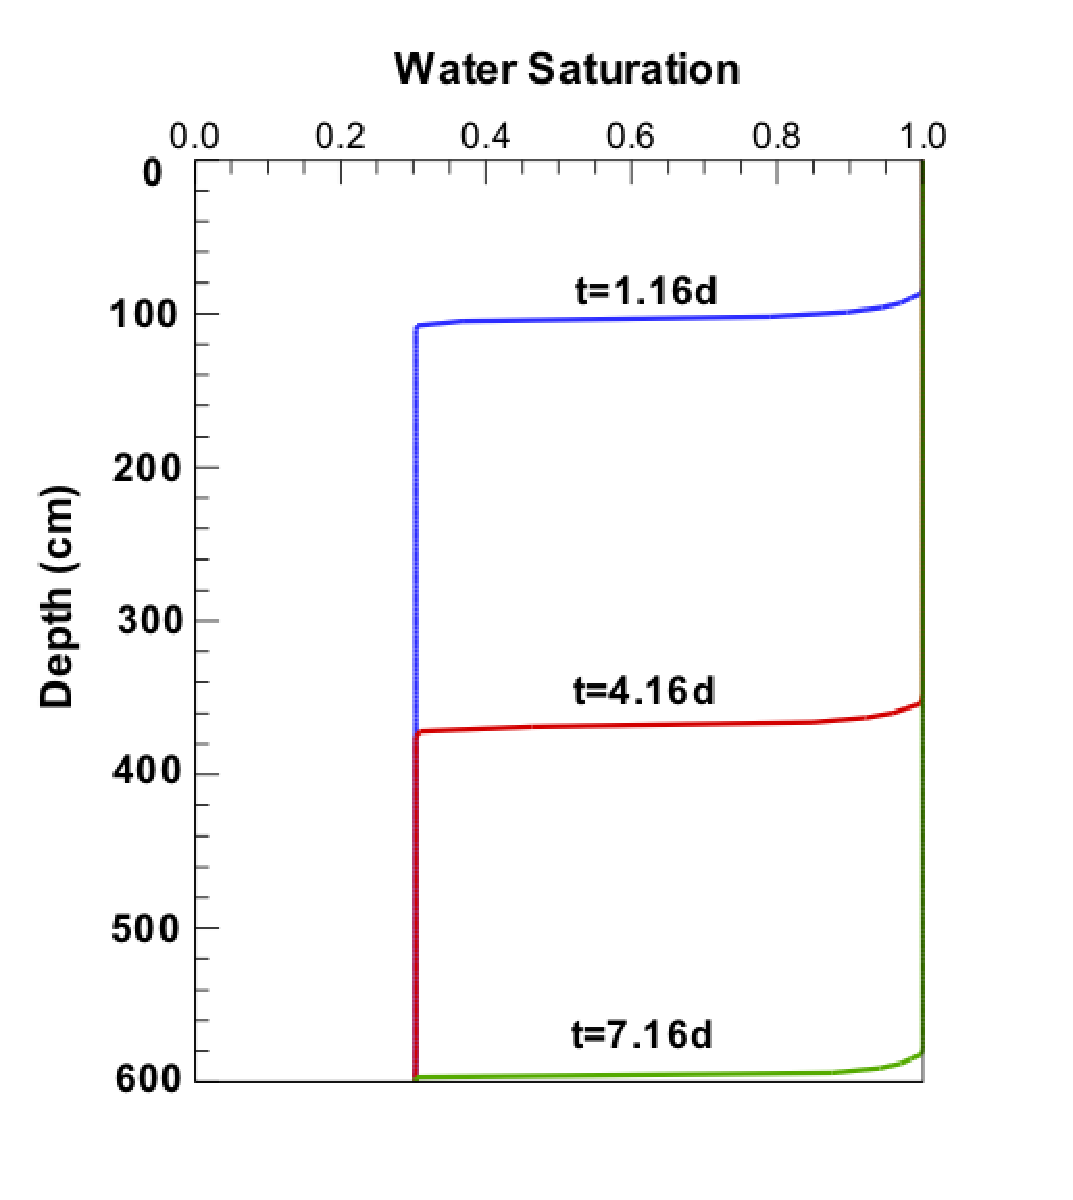
\includegraphics[height=0.85\columnwidth, angle=0]{H_US/figures/result_forsyth.eps}
\end{picture}
\end{minipage}
%
\caption{Saturation simulation by \cite{Forsyth:1995} and GeoSys }
\label{us:result-forsyth}
\end{figure}
%-------------------------------------------------
\subsubsection*{Benchmark deposit}
\begin{tabular}{|l|l|l|}
  \hline
  Benchmark & Problem type & Path in benchmark deposit \\
  \hline
 \emph{h\_us\_line\_forsyth} & H & benchmarks\verb \h_us\wet\ \\
   \hline
\end{tabular}
%
\subsection{Infiltration in homogenous soil (BC/BC)}
\subsubsection*{Problem definition}
Numerical results compare with classical experimental measurements
of Celia et al.(1990). The soil column is 0.6m long. The problem
is defined as uniform initial condition in water head, fixed water
head at top, van Genuchten homogenous material and constant mesh
density.
%
\subsubsection*{Initial, boundary conditions and source term}
The initial condition of pressure is -10m, and boundary conditions
at top and bottom are -0.75m and -10m. Details are illustrated in
Fig. \ref{us:celia}.
%
%-------------------------------------------------
\begin{figure} [h]
 \centering
 \includegraphics[width=0.20\columnwidth] {H_US/figures/illustration_celia.eps}
 \caption{Illustration of numerical model}
 \label{us:celia}
\end{figure}
%-------------------------------------------------
\subsubsection*{Material properties}
Homogenous material properties are assumed within the whole
domain. Table \ref{us:celia-setting} gives the parameters.
%------------------------------
\begin{table}[H]
 \centering
 \caption{Parameters in simulation} \centering \label{us:celia-setting}
 \begin{tabular}{llll}
 \hline\hline\noalign{\smallskip}
 Parameter    & Value  &  Unit  \\ \hline
 Porosity          & 0.368   & -   \\
 Saturated permeability $k_s$ & 9.35247e-12 & $m^2$  \\
 $S_r^l$           & 0.277    &  - \\
 $S_{max}^l$        & 1.0    &  - \\
 $\alpha$           & 3.35   &  $1/m$ \\
 $n$                & 2      &  - \\
 Gravity constant $g$ & 9.807      &  $m/s^2$ \\
 Liquid density $\rho$ & 998.2     &  $kg/m^3$ \\
\noalign{\smallskip}\hline\hline
 \end{tabular}
\end{table}
%------------------------------
\subsubsection*{Results}
Fig. \ref{us:result-celia} shows the distribution of saturation.
Left side in Fig.\ref{us:result-celia} is the result of reference.
In GeoSys/RockFlow the tangent approximation is used.
%-------------------------------------------------
\begin{figure}[h]
\centering \vspace{1cm} \unitlength1cm
\begin{minipage}[t]{5.8cm}
\begin{picture}(5.8, 4.4)
\includegraphics[height=0.9\columnwidth, angle=0]{H_US/figures/Reference_celia.eps}
\end{picture}\par
\end{minipage}
\hfill
\begin{minipage}[t]{5.4cm}
\unitlength1cm
\begin{picture}(5.4, 4.1)
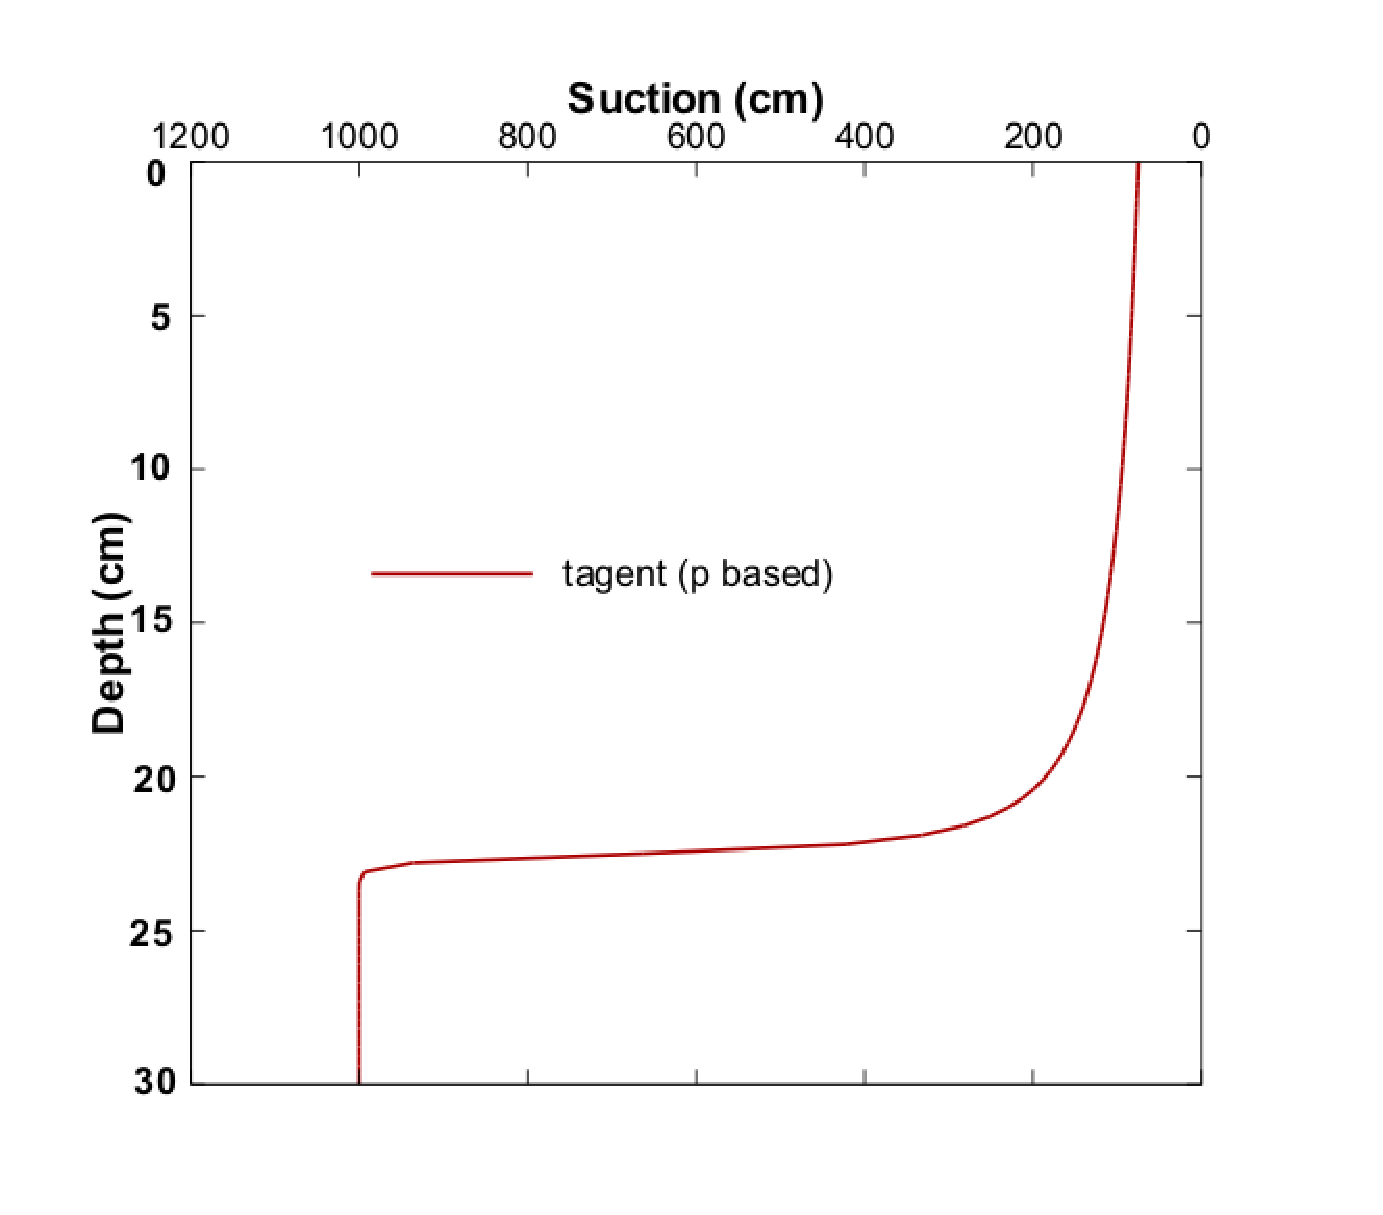
\includegraphics[height=0.9\columnwidth, angle=0]{H_US/figures/result_celia.eps}
\end{picture}
\end{minipage}
%\begin{center}
%\hspace{0.0cm} (a) \hspace{6.0cm} (b)
%\end{center}
\caption{Suction distribution simulation by \cite{Rathfeder:1994}
and GeoSys at 6 hours} \label{us:result-celia}
\end{figure}

%-------------------------------------------------
\subsection{Transient infiltration in homogenous soil}

\subsubsection*{Problem definition}

This study case comes from David Kuntz in Tübingen, and it is
compared with the numerical solutions of Min3P. It is a 0.25
length soil column with an artificial transient water discharge at
top. Three points are selected at different location of the
column, and the saturation evolution are presented. The
description of model is
shown in Fig. \ref{us:illu-transient}.\\
%-------------------------------------------------
\begin{figure} [h]
 \centering
 \includegraphics[width=0.30\columnwidth] {H_US/figures/illustration_Transient.eps}
 \caption{Illustration of numerical model}
 \label{us:illu-transient}
\end{figure}
%-------------------------------------------------

\subsubsection*{Initial, boundary conditions and source term}
The initial condition is set by restart file. Artificial transient
infiltration source term at top instead of boundary
condition,which is shown in Fig. \ref{us:dischargetransient}.
Fixed boundary condition at bottom as pressure equal -31800Pa.\\

%-------------------------------------------------
\begin{figure} [h]
 \centering
 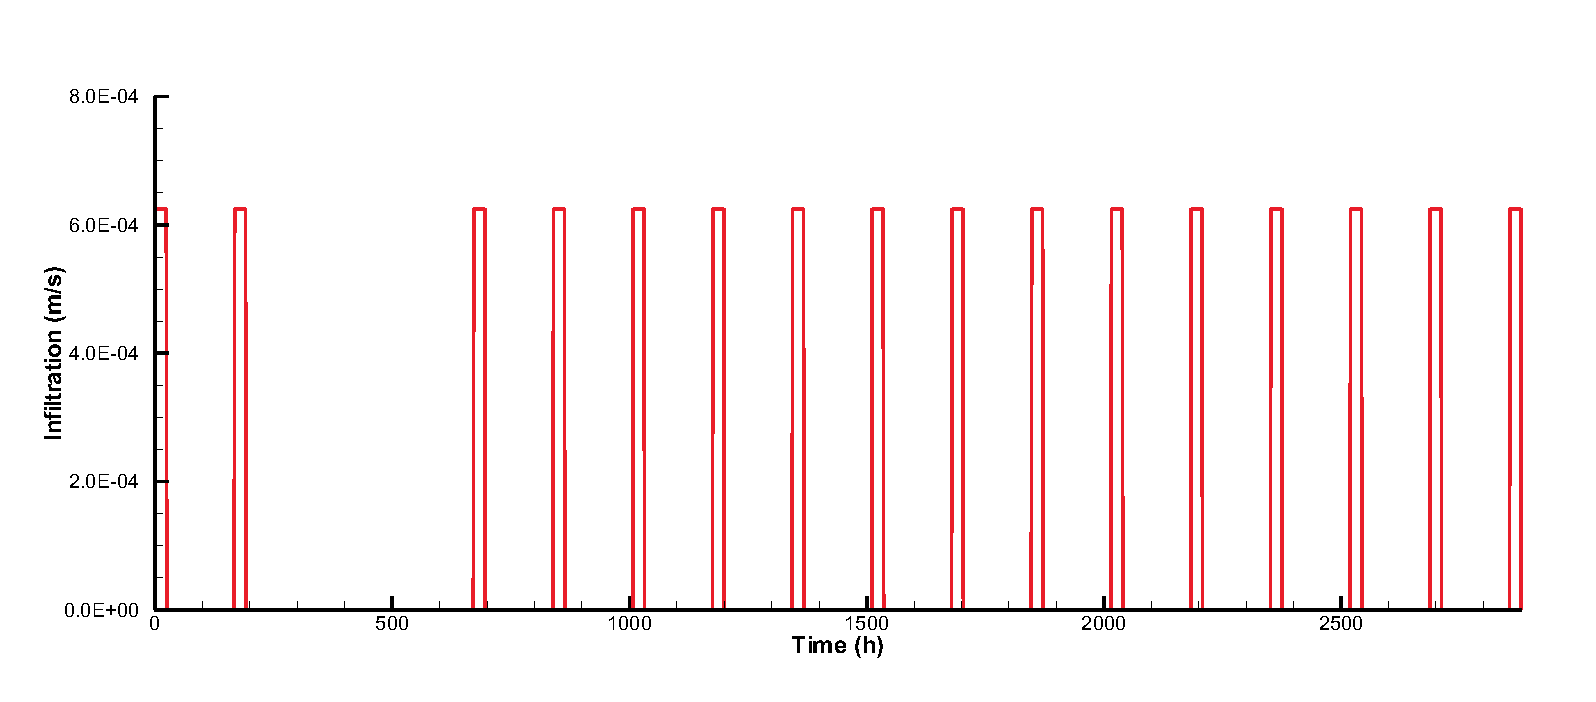
\includegraphics[width=0.8\columnwidth] {H_US/figures/discharge_transient.eps}
 \caption{Discharge serial at the top}
 \label{us:dischargetransient}
\end{figure}
%-------------------------------------------------

\subsubsection*{Material properties}
Homogeneous material is defined by van Genuchten parameters and
Table \ref{us:transientsetting} gives the parameters.
%------------------------------
\begin{table}[H]
 \centering
 \caption{Parameters in simulation} \centering \label{us:transientsetting}
 \begin{tabular}{llll}
 \hline\hline\noalign{\smallskip}
 Parameter    & Value  &  Unit  \\ \hline
 Porosity          & 0.406   & -   \\
 Saturated permeability $k_s$ & 9.35247e-12 & $m^2$  \\
 $S_r^l$           & 0.056    &  - \\
 $S_{max}^l$        & 1.0    &  - \\
 $\alpha$           & 4.56   &  $1/m$ \\
 $m$                & 0.254      &  - \\
 Gravity constant $g$ & 9.8      &  $m/s^2$ \\
 Liquid density $\rho$ & 1000     &  $kg/m^3$ \\
\noalign{\smallskip}\hline\hline
 \end{tabular}
\end{table}
%------------------------------
\subsubsection*{Results}
The vertical distributions of saturation at some moments are shown
in Fig.\ref{us:result-transient}.\\
%
\begin{figure} [h]
 \centering
 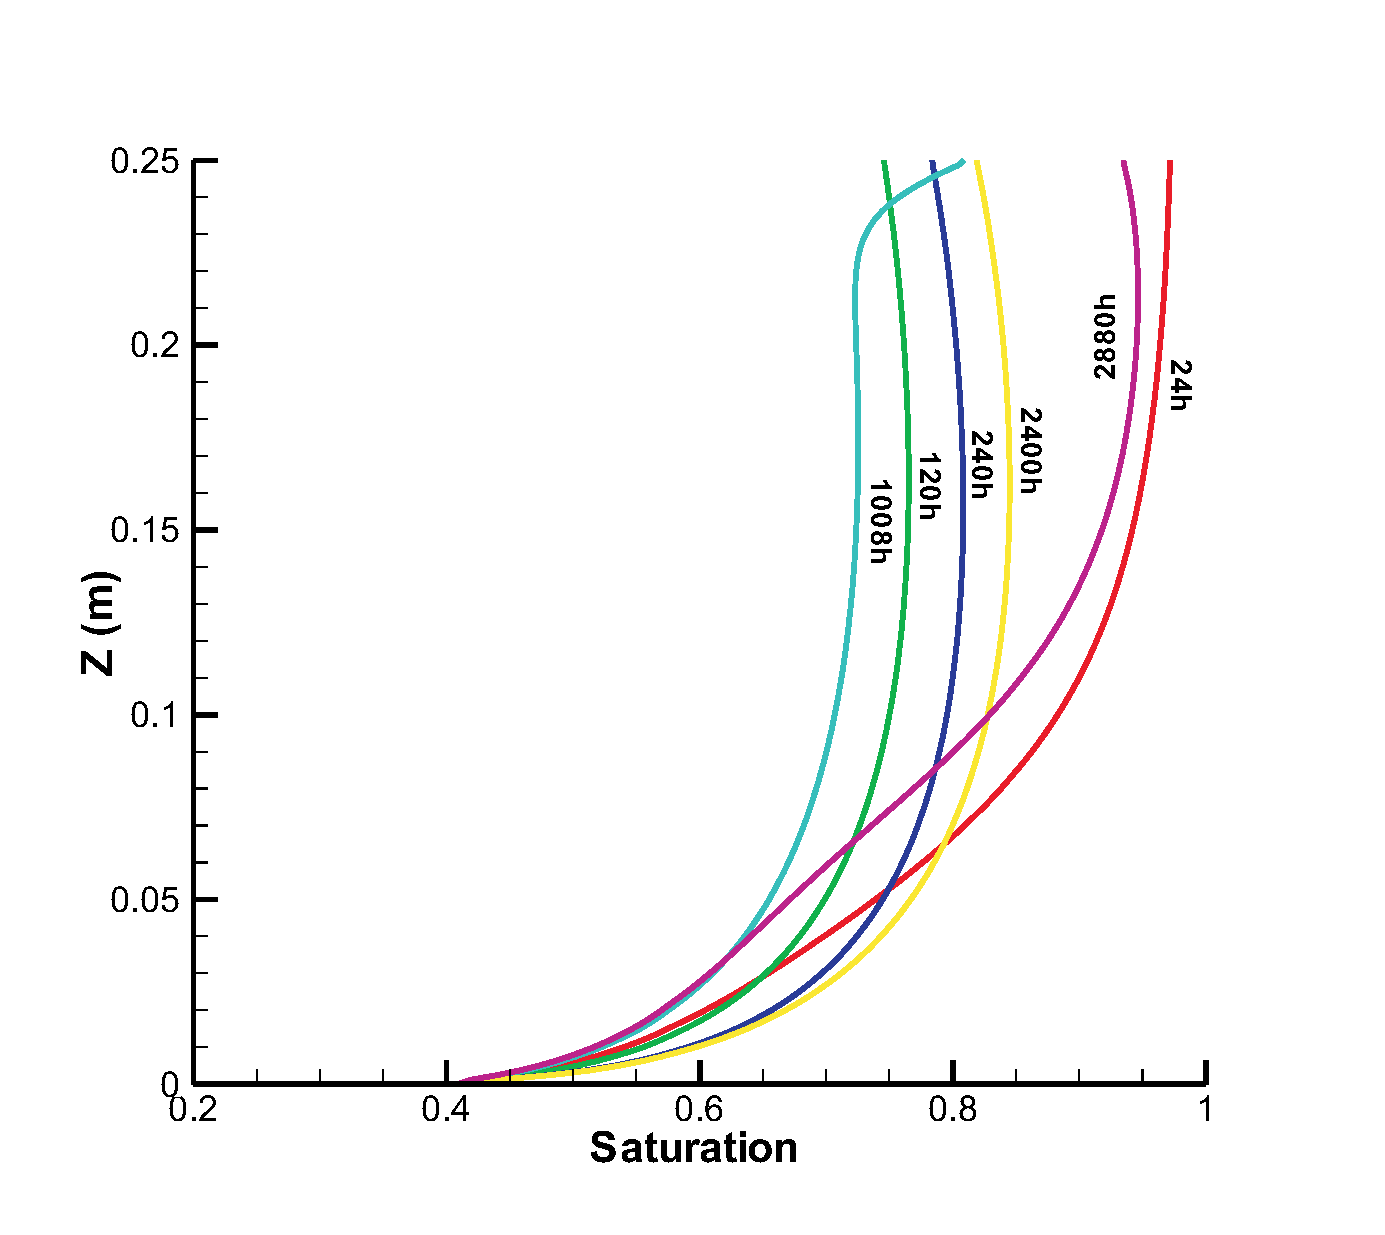
\includegraphics[width=0.60\columnwidth] {H_US/figures/result_transient.eps}
 \caption{Saturation distributions}
 \label{us:result-transient}
\end{figure}
%
Three points, which locate at (0,0,0.25),(0,0,0.10) and (0,0,0.05)
respectively, are selected to see the time evolution of saturation
and compare with those by Min3p. Fig.\ref{us:comparisonMin3p}
shown the results.\\
%
\begin{figure} [h]
 \centering
 \includegraphics[width=0.60\columnwidth] {H_US/figures/Transient_withMin3p.eps}
 \caption{comparison of saturation time evolutions
 three points}
 \label{us:comparisonMin3p}
\end{figure}
%
\subsubsection*{Benchmark deposit}
\begin{tabular}{|l|l|l|}
  \hline
  Benchmark & Problem type & Path in benchmark deposit \\
  \hline
 \emph{Transient} & H & benchmarks\verb \h_us\wet\ \\
  \hline
\end{tabular}
%

\subsection{Nouniform IC of heterogenous soil column (-/BC)}
%
\subsubsection*{Problem definition}
The case is from DECOVALEX.  Heterogenous horizontal soil column
starts at nouniform status, and results show the interruptions at
the interface of two material.
%
\subsubsection*{Initial and boundary conditions}
Heterogeneous initial condition setting is loaded by restart file,
and fixed boundary condition is at the end. Details are
illustrated in Fig. \ref{us:DECO}.
%-------------------------------------------------
\begin{figure} [h]
 \centering
 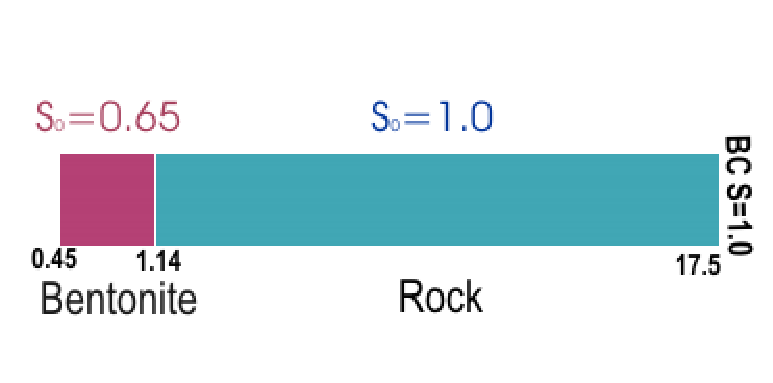
\includegraphics[width=0.45\columnwidth] {H_US/figures/illustration_DECO.eps}
 \caption{Illustration of numerical model}
 \label{us:DECO}
\end{figure}
%-------------------------------------------------
\subsubsection*{Material properties}
The heterogeneous soil column consists of two kinds material:
bentonite and rock. The ven Genuchten parameters of rock are shown
in Tab.\ref{us:DECOVALEX-setting}, and as for bentonite the curves
in Fig. \ref{us:curve-DECO} are used in the simulation.
%------------------------------
\begin{table}[H]
 \centering
 \caption{Parameters in DECOVALEX}
 \centering \label{us:DECOVALEX-setting}
 \begin{tabular}{llll}
 \hline\hline\noalign{\smallskip}
 Parameter    & Rock  &   Bentonite  &  Unit  \\ \hline
 Porosity     & 0.41  &   0.01   & -   \\
 Saturated permeability $k_s$ & 1.03e-17 & 2.0e-21 & $m^2$ \\
 $S_r^l$           & 0       &  -  & -\\
 $S_{max}^l$       & 1.0     &  -  & -\\
 $\alpha$          & 6.673   &  -  & $1/m$ \\
 $n$               & 0.6     &  -  & -\\
\noalign{\smallskip}\hline\hline \\
 \end{tabular}
\end{table}
%------------------------------
\begin{figure} [h]
 \centering
 \includegraphics[width=0.60\columnwidth] {H_US/figures/DECOVALEXmaterial.eps}
 \caption{Characteristic Curves for bentonite and granite rock}
 \label{us:curve-DECO}
\end{figure}
%
%------------------------------
\subsubsection*{Results}
 Fig. \ref{us:result-DECO}
shows the distribution of saturation and pressure.
%-------------------------------------------------
\begin{figure}[h]
\centering \vspace{0.0cm} \unitlength 1cm
\begin{minipage}[t]{6 cm}
\begin{picture}(6,5)
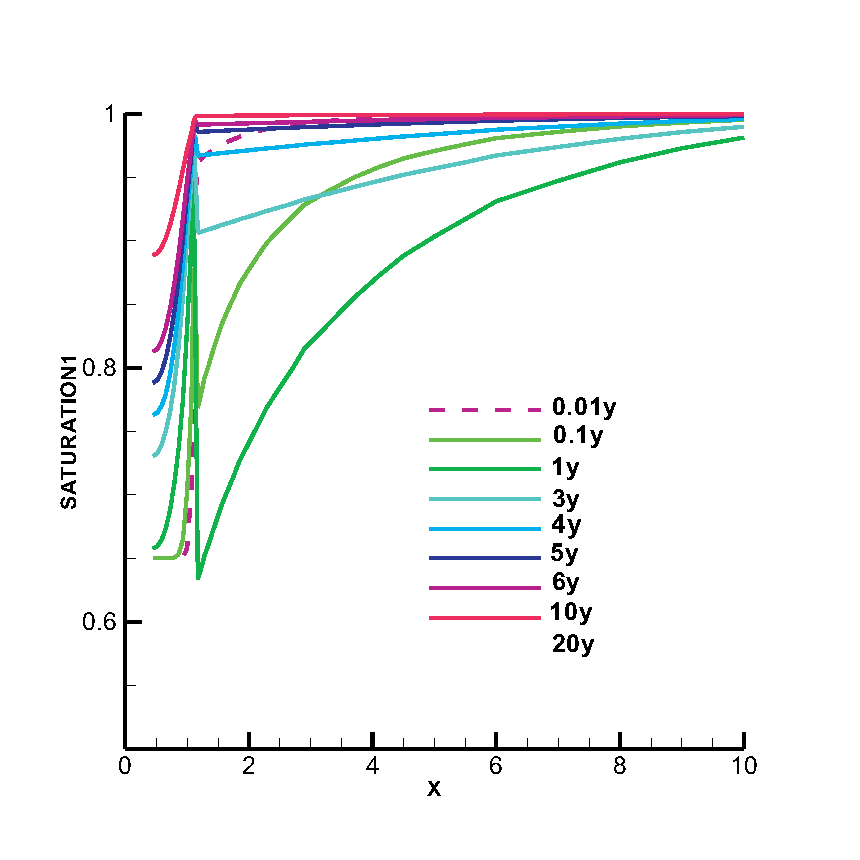
\includegraphics[height=0.90\columnwidth, angle=0]{H_US/figures/result_1ho_S.eps}
\end{picture}\par
\end{minipage}
\hfill
\begin{minipage}[t]{6 cm}
\unitlength1cm
\begin{picture}(6,5)
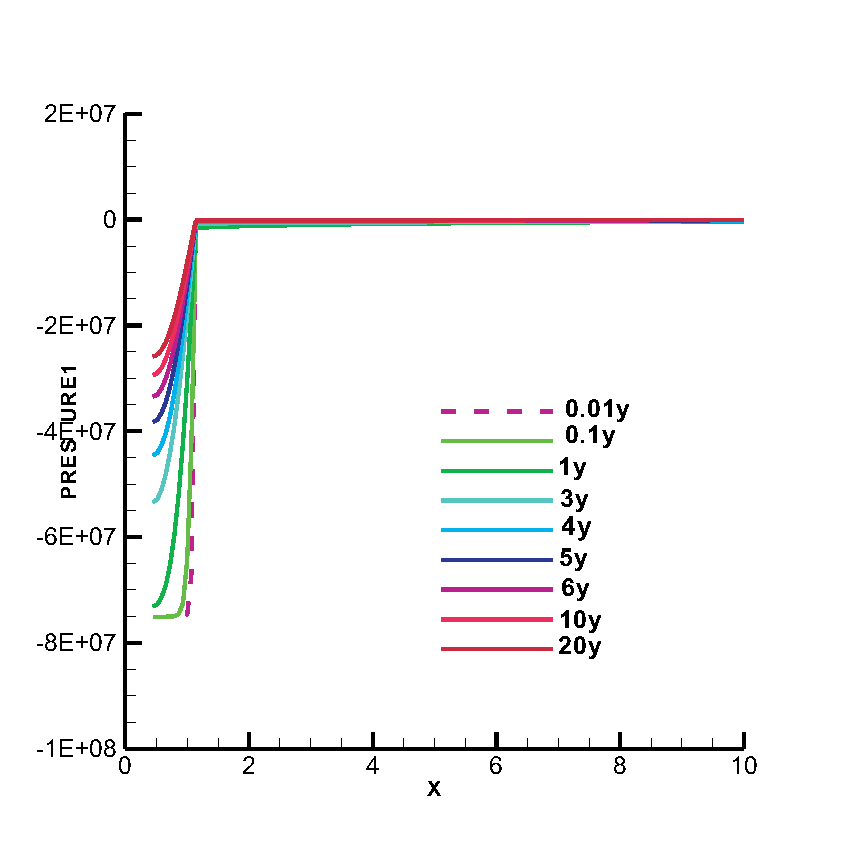
\includegraphics[height=0.90\columnwidth, angle=0]{H_US/figures/result_1ho_P.eps}
\end{picture}
\end{minipage}
%\begin{center}
%\hspace{0.0cm} (a) \hspace{6.0cm} (b)
%\end{center}
\caption{Saturation and pressure distribution}
\label{us:result-DECO}
\end{figure}
%-------------------------------------------------
\subsubsection*{Benchmark deposit}
\begin{tabular}{|l|l|l|}
  \hline
  Benchmark & Problem type & Path in benchmark deposit \\
  \hline
 \emph{1d\_ho} & H & benchmarks\verb \h_us\wet\ \\
   \hline
\end{tabular}
%
%\subsection{Unsaturated flow: Liakopoulos Experiment}
%\subsubsection*{Problem definition}
%It is a drainage test based on an experiment by Liakopoulos(1965).
%The detail problem definition can be seen in HM processes section
%\ref{sec:Liakopoulos}, the results of coupled hydraulic process
%(H) and deformation process (M) are presented. Here the single H
%process are simulated without M, and the results are in
%comparisons with HM in section \ref{sec:Liakopoulos} Fig.
%\ref{fig:H-US}.
%
%\subsubsection*{Benchmark deposit}
%\begin{tabular}{|l|l|l|}
%  \hline
%  Benchmark & Problem type & Path in benchmark deposit \\
%  \hline
% \emph{h\_us\_line\_drainage} & H & benchmarks\verb \h_us\drainage\ \\
%   \hline
%\end{tabular}

\section{Dual continua}
Dual continua model is based on Eq. \ref{eqn:pbased_m} and
\ref{eqn:pbased_f}.
\subsection{Comparison with S1D}
\label{dual-1}
\subsubsection*{Problem definition}
The simple case is defined by Vogel (2007)\cite{vogel:2007}.
Numerical results compare with HYDRUS for single continua and S1D
for dual continua model.
%
\subsubsection*{Initial and boundary conditions}
The initial conditions for both matrix and fracture continuum are
identical as a gradient pressure distribution, which are
$p^l_{top}$ = -27440$Pa$ and $p^l_{bottom}$ = -21560$Pa$. The
boundary conditions for both continua are also identical as fixed
BC at top $p^l_{top}$ = 98$Pa$ and free drainage at bottom.
Details are illustrated in Fig. \ref{us:dual-1d}.
%-------------------------------------------------
\begin{figure} [h]
 \centering
 \includegraphics[width=0.4\columnwidth] {H_US/figures/illustration_dual_1D.eps}
 \caption{Illustration of numerical model}
 \label{us:dual-1d}
\end{figure}
%-------------------------------------------------
\subsubsection*{Material properties}
Table \ref{us:Dual-line-setting} gives the parameters
%------------------------------
%\begin{table}[H]
% \centering
% \caption{Parameters in simulation}
% \centering \label{us:Dual-line-setting}
% \begin{tabular}{llll}
% \hline\hline\noalign{\smallskip}
% Soil type       & Items    & Setting  & Original setting  \\ \hline
%                 &  Preferential factor   & 0.95    & 0.95\\
%Matrix           &  Porosity              & 0.498   & 0.498\\
%continuum        &  $S_r^l$               & 0.0     & 0.0 \\
%                 &  $S_{max}^l$           & 1.0     & 1.0 \\
%                 &  $\alpha$ $(1/m)$      & 1.8     & 1.8  \\
%                 &  $n$                   & 1.8     & 1.8 \\
%                 &  Saturated permeability($1/m^2$) & 2.32368E-13 & 2.32368E-13 \\
%\hline
%                 &  Preferential factor   & 0.05  & 0.05  \\
%                 &  Porosity           & 0.6      & 0.6  \\
%Fracture         &  $S_r^l$            & 0.0833   & 0.0833 \\
%continuum        &  $S_{max}^l$        & 1.0      & 1.0   \\
%                 &  $\alpha$ $(1/m)$   & 5.6      & 14.5    \\
%                 &  $n$                & 2.68     & 2.68 \\
%                 &  Saturated permeability($1/m^2$) & 1.09000E-11 & 1.29781E-11\\
%\hline
% Transfer    &  Transfer coefficient$(1/m^2)$  &  500  &  500 \\
% \noalign{\smallskip}\hline\hline
% \end{tabular}
%\end{table}
%------------------------------
%------------------------------
\begin{table}[H]
 \centering
 \caption{Parameters in simulation}
 \centering \label{us:Dual-line-setting}
 \begin{tabular}{llll}
 \hline\hline\noalign{\smallskip}
 Soil type       & Items    & Setting   \\ \hline
                 &  Preferential factor   & 0.95    \\
Matrix           &  Porosity              & 0.498   \\
continuum        &  $S_r^l$               & 0.0    \\
                 &  $S_{max}^l$           & 1.0      \\
                 &  $\alpha$ $(1/m)$      & 1.8       \\
                 &  $n$                   & 1.8     \\
                 &  Saturated permeability($1/m^2$) & 2.32368E-13  \\
\hline
                 &  Preferential factor   & 0.05   \\
                 &  Porosity           & 0.6       \\
Fracture         &  $S_r^l$            & 0.0833    \\
continuum        &  $S_{max}^l$        & 1.0       \\
                 &  $\alpha$ $(1/m)$   & 5.6       \\
                 &  $n$                & 2.68      \\
                 &  Saturated permeability($1/m^2$) & 1.09000E-11 \\
\hline
 Transfer    &  Transfer coefficient$(1/m^2)$  &  500  \\
 \noalign{\smallskip}\hline\hline
 \end{tabular}
\end{table}
%------------------------------
\subsubsection*{Results}
Fig. \ref{us:result-dual-line-c1} shows the pressure distribution
comparison of single continuum at the time of 20 min and 30 min,
which are calculated by GeoSys/RlockFlow (lines) and HYDRUS
(symbols) respectively. The solid lines are pressure fronts of
matrix, and the dash lines are fracture.
%-------------------------------------------------
\begin{figure} [htb!]
 \centering
 \includegraphics[width=0.75\columnwidth] {H_US/figures/dual_single.eps}
 \caption{Pressure comparison of two single continua}
 \label{us:result-dual-line-c1}
\end{figure}
%-------------------------------------------------
The comparisons of dual-continua model results are shown in Fig.
\ref{us:result-dual-line-c2}. The blue lines are the outcomes
without transfer term, and the red lines by GeoSys/RockFlow and
symbols by S1D show the exchange effects within two continua.
Since matrix continuum is the dominant part in whole system, and
the influence on matrix is less than that on fracture.

%-------------------------------------------------
\begin{figure} [htb!]
 \centering
 \includegraphics[width=0.75\columnwidth] {H_US/figures/dual_coupled.eps}
 \caption{Pressure comparison of DPM}
 \label{us:result-dual-line-c2}
\end{figure}
%-------------------------------------------------
\subsubsection*{Benchmark deposit}
\begin{tabular}{|l|l|l|}
  \hline
  Benchmark & Problem type & Path in benchmark deposit \\
  \hline
 \emph{dual\_vl} & H & benchmarks\verb \h_us\dual\ \\
   \hline
\end{tabular}

%-------------------------------------------------

\subsection{Classic case: Gerke. etc}
 \label{dual-2}
\subsubsection*{Problem definition}
The section is a dual continua model comparison of GeoSys/RockFlow
with the paper work of Gerke(1993)\cite{Gerke:1993}.
%
\subsubsection*{Initial and boundary conditions}
The initial conditions for both matrix and fracture continuum are
identical, which are set as $h^l_m$ = $h^l_f$ =-10$m$ and $p^l_m$
= $p^l_f$ =-9800$Pa$ in GeoSys/RockFlow. The infiltration
exclusively goes into the fracture pore part, matrix continuum
gets water from transfer. Details are illustrated in Fig.
\ref{us:dual-1d}.
%-------------------------------------------------
\begin{figure} [h]
 \centering
 \includegraphics[width=0.2\columnwidth] {H_US/figures/illustration_dual_1D2.eps}
 \caption{Illustration of numerical model}
 \label{us:dual-1d}
\end{figure}
%-------------------------------------------------
\subsubsection*{Material properties}
Table \ref{us:Dual-line-setting2} gives the parameters
%------------------------------
\begin{table}[H]
 \centering
 \caption{Parameters in simulation}
 \centering \label{us:Dual-line-setting2}
 \begin{tabular}{llll}
 \hline\hline\noalign{\smallskip}
 Soil type       & Items    & Setting  \\ \hline
                 &  Preferential factor   & 0.95   \\
Matrix           &  Porosity              & 0.5   \\
continuum        &  $S_r^l$               & 0.21052    \\
                 &  $S_{max}^l$           & 1.0      \\
                 &  $\alpha$ $(1/m)$      & 0.05       \\
                 &  $n$                   & 1.5    \\
                 &  Saturated permeability($1/m^2$) & 1.2419E-14  \\
\hline
                 &  Preferential factor   & 0.05    \\
                 &  Porosity           & 0.5      \\
Fracture         &  $S_r^l$            & 0.0    \\
continuum        &  $S_{max}^l$        & 1.0       \\
                 &  $\alpha$ $(1/m)$   & 5.6     \\
                 &  $n$                & 10    \\
                 &  Saturated permeability($1/m^2$) & 2.3596E-11\\
\hline
 Transfer    &  Transfer coefficient$(1/m^2)$  &  $0.01\times0.5[K(p_m)+K(p_f)]$ \\
 \noalign{\smallskip}\hline\hline
 \end{tabular}
\end{table}
%------------------------------
\subsubsection*{Results}
Fig. \ref{us:result-dual-van} shows simulated pressure and
saturation profiles during infiltration at some time steps.
%-------------------------------------------------
\begin{figure}[h]
\centering \vspace{1cm} \unitlength1cm
\begin{minipage}[t]{6 cm}
\begin{picture}(6,5)
\includegraphics[height=0.9\columnwidth, angle=0]{H_US/figures/dual_van_p.eps}
\end{picture}\par
\end{minipage}
\hfill
\begin{minipage}[t]{6cm}
\unitlength1cm
\begin{picture}(6,5)
\includegraphics[height=0.9\columnwidth, angle=0]{H_US/figures/dual_van_S.eps}
\end{picture}
\end{minipage}
%\begin{center}
%\hspace{0.0cm} (a) \hspace{6.0cm} (b)
%\end{center}
\caption{Simulated pressure and saturation profiles of the matrix
(solid lines) and fracture (dashed lines)}
\label{us:result-dual-van}
\end{figure}
%-------------------------------------------------
\subsubsection*{Benchmark deposit}
\begin{tabular}{|l|l|l|}
  \hline
  Benchmark & Problem type & Path in benchmark deposit \\
  \hline
 \emph{dual\_van} & H & benchmarks\verb \h_us\dual\ \\
   \hline
\end{tabular}
%
\subsection{Discussion}
\begin{description}
  \item The pressure evolution of fracture continuum in
  \ref{dual-1} calculated by GeoSys/RlockFlow is a little slower than that by
  HYDRUS.
  \item  The distributions of saturation and pressure in \ref{dual-2}
  are different from the paper. The saturation of
  fracture is $S\in[0,0.05]$ in \cite{Gerke:1993}.
%
\end{description}
%

\section{Regional soil model}
\subsubsection*{Problem definition}
For the large scale area, soil represent significant
diversification of moisture content with respect to the
meteorologic changing such as precipitation and evapotranspiration
as well as its physically-based continuum mechanics. Coupled
hydrologic model with global climate model (GCM) is developed to
research the impact of climate variabilities to vadose zone. The
responses and water budget of alterations in timing and
distribution of precipitation on the unsaturated zone are focused
on by deterministic physically-based RSM, which is flexible and
adaptable to extent one dimensional vertical column to three
dimensional spatial area according to the heterogenous
characteristics of climatological conditions, soil properties,
geographic elevation, which is shown in Fig.\ref{us:RSMmodelconcept}. \\
%------------------------------------------
\begin{figure}[htb!]
  \center
  \includegraphics[width=0.6\textwidth]{H_US/figures/RSMconcept.eps}
  \caption{Concept of regional soil model}
  \label{us:RSMmodelconcept}
\end{figure}
%------------------------------------------
\subsubsection*{Initial and boundary conditions}
Initial condition in the whole domain is set as: $P^l=-9000.0 Pa$,
and the top BC is set as pure infiltration serial in 2000 year in
Beerze-Reusel basin, which is described by functions (FCT).

\subsubsection*{Material properties}
The soil materials are from Beerze-Reusel drainage basin. There
are several different soil types representing sand, loam and peat
soils formed during the pleistocene, and those soil compose 5
kinds of soil profile type, which are defined the vertical
structure of soil column. The soil water characteristic curves
(SWCC) are given to describe the different soil properties (Fig.
\ref{fig:soil_columns}, left), for complete SSWC descriptions for
the investigation area can be found in \cite{DuEtAl:2006}.
%
\subsubsection*{Results}
The saturation evolutions of selected soil columns are shown in
Fig. \ref{fig:soil_columns} (right).
%
\begin{figure}[htb!]
  \begin{center}
    \begin{minipage}[t]{0.45\textwidth}
      \begin{center}
        \includegraphics[scale=0.27]{H_US/figures/Soil_P1.eps}
      \end{center}
    \end{minipage}
  %%\hspace{0.01\textwidth}
    \begin{minipage}[t]{0.45\textwidth}
      \begin{center}
        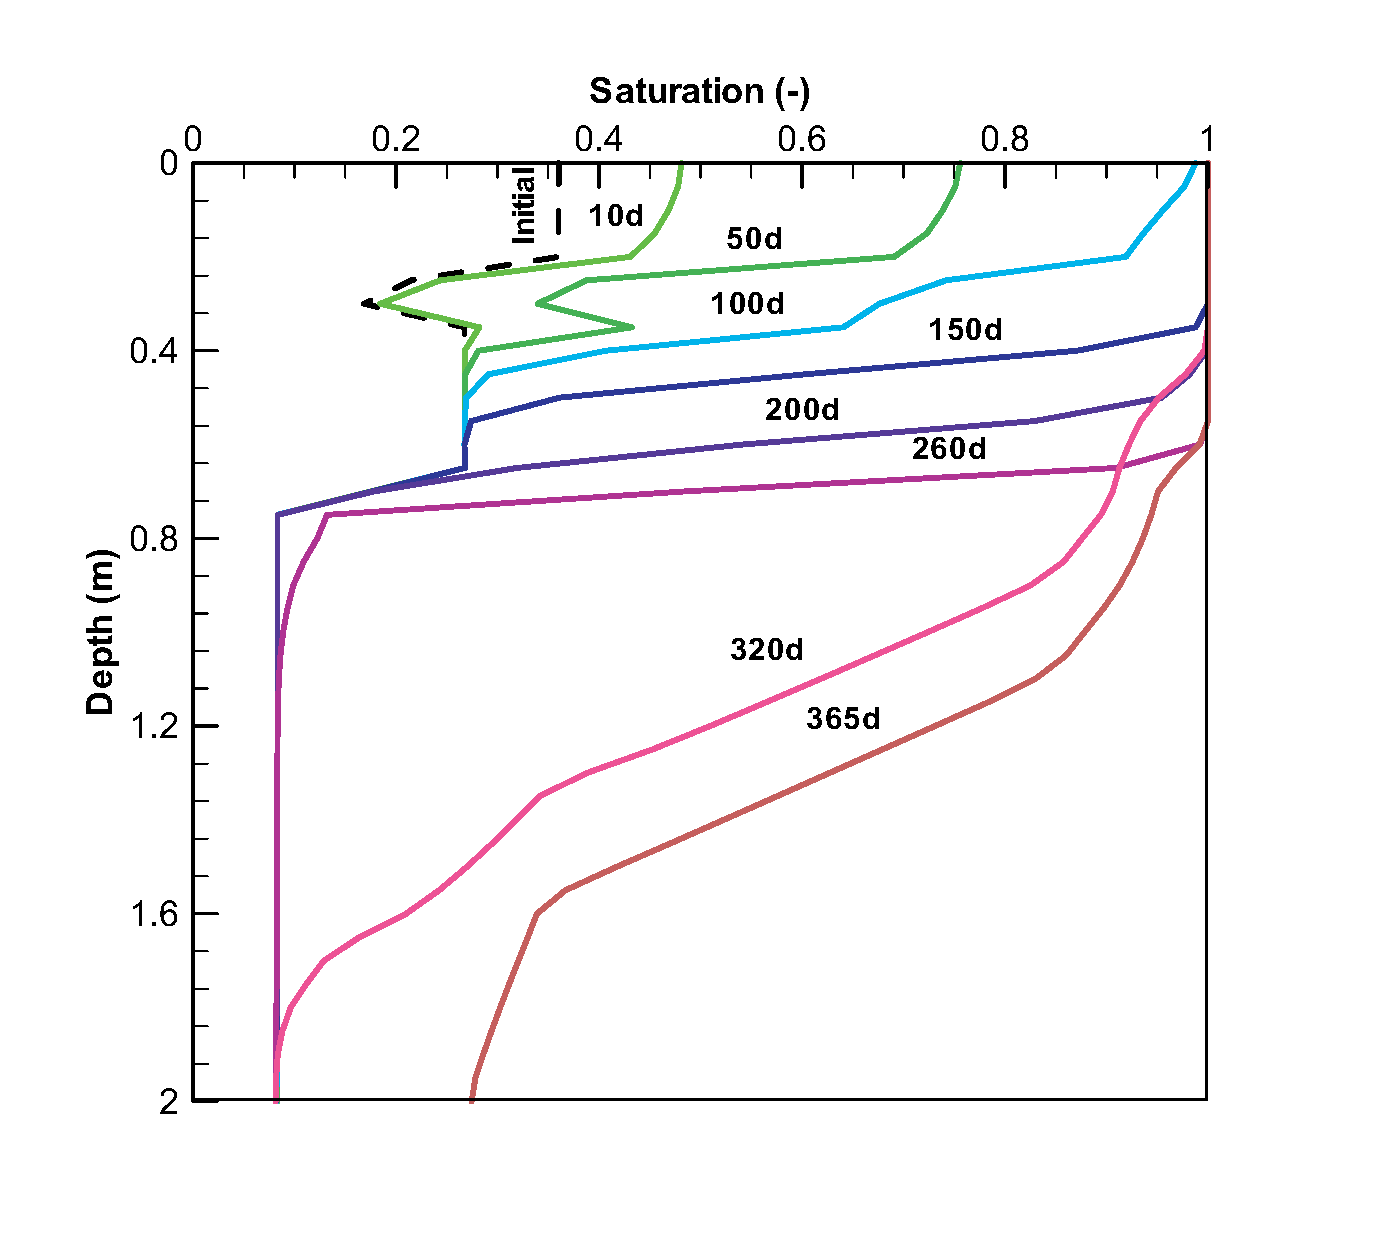
\includegraphics[scale=0.27]{H_US/figures/pl1_s.eps}
      \end{center}
    \end{minipage}\\
  \end{center}
%
  \begin{center}
    \begin{minipage}[t]{0.45\textwidth}
      \begin{center}
        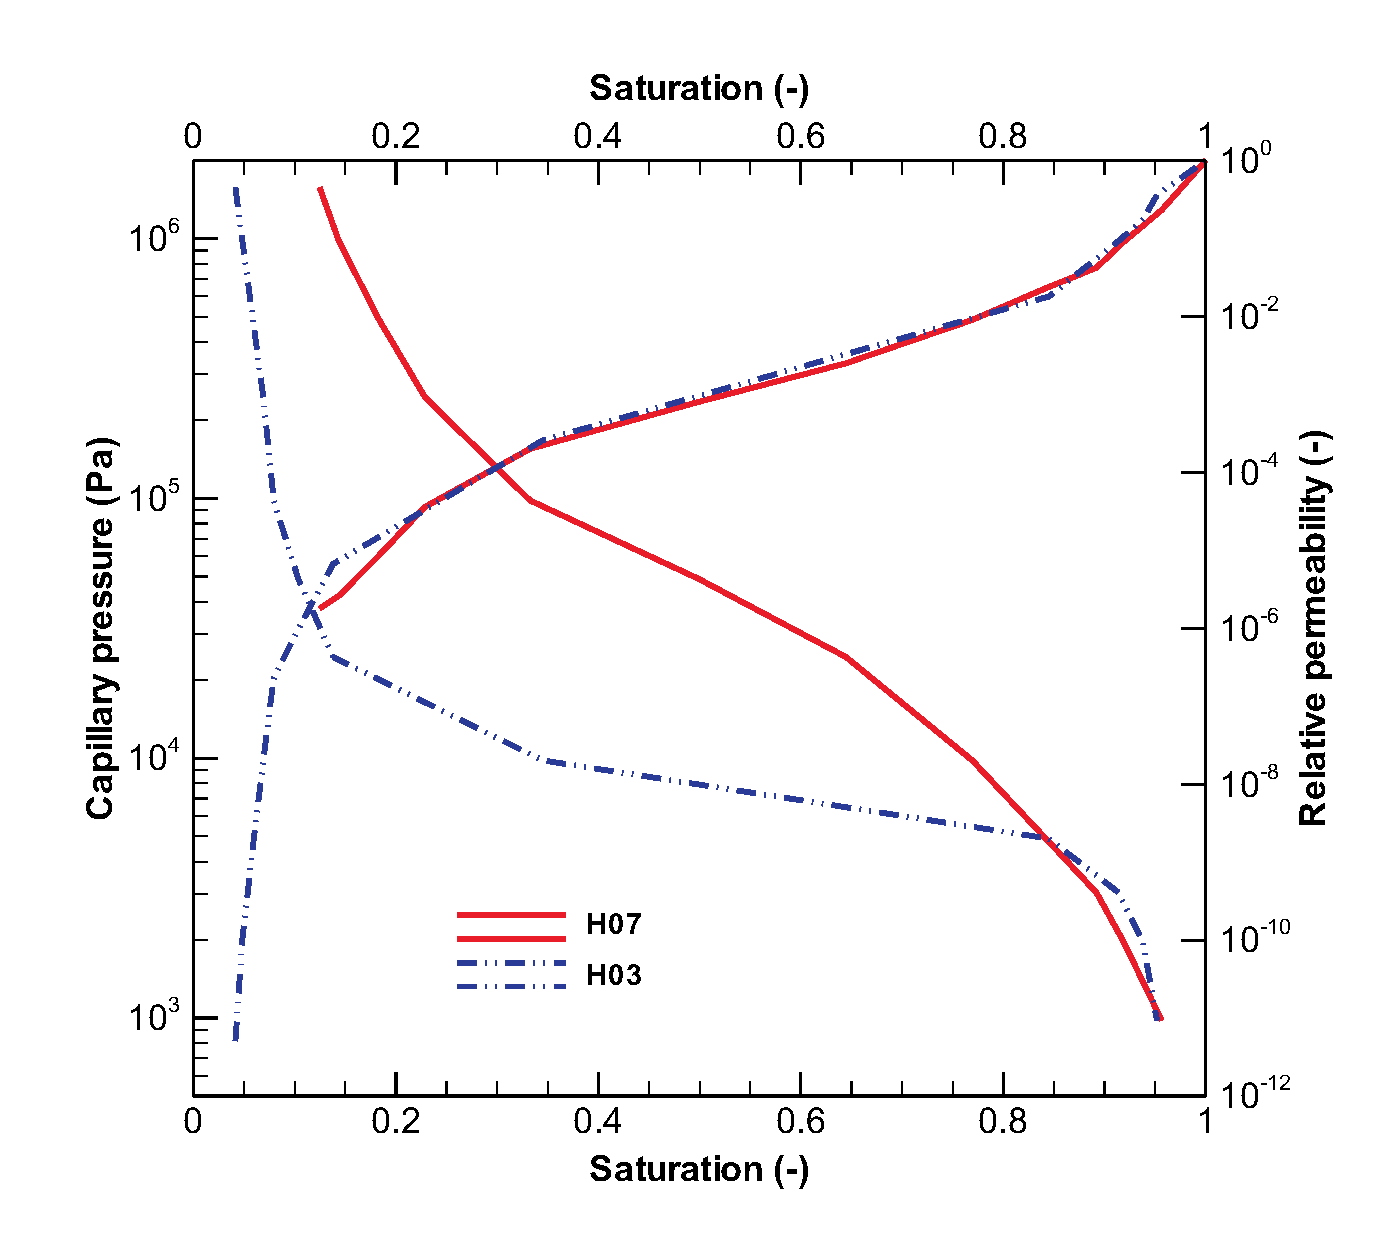
\includegraphics[scale=0.27]{H_US/figures/Soil_P2.eps}
      \end{center}
    \end{minipage}
  %%\hspace{0.01\textwidth}
    \begin{minipage}[t]{0.45\textwidth}
      \begin{center}
        \includegraphics[scale=0.27]{H_US/figures/pl2_s.eps}
      \end{center}
    \end{minipage}\\
  \end{center}
%
  \begin{center}
    \begin{minipage}[t]{0.45\textwidth}
      \begin{center}
        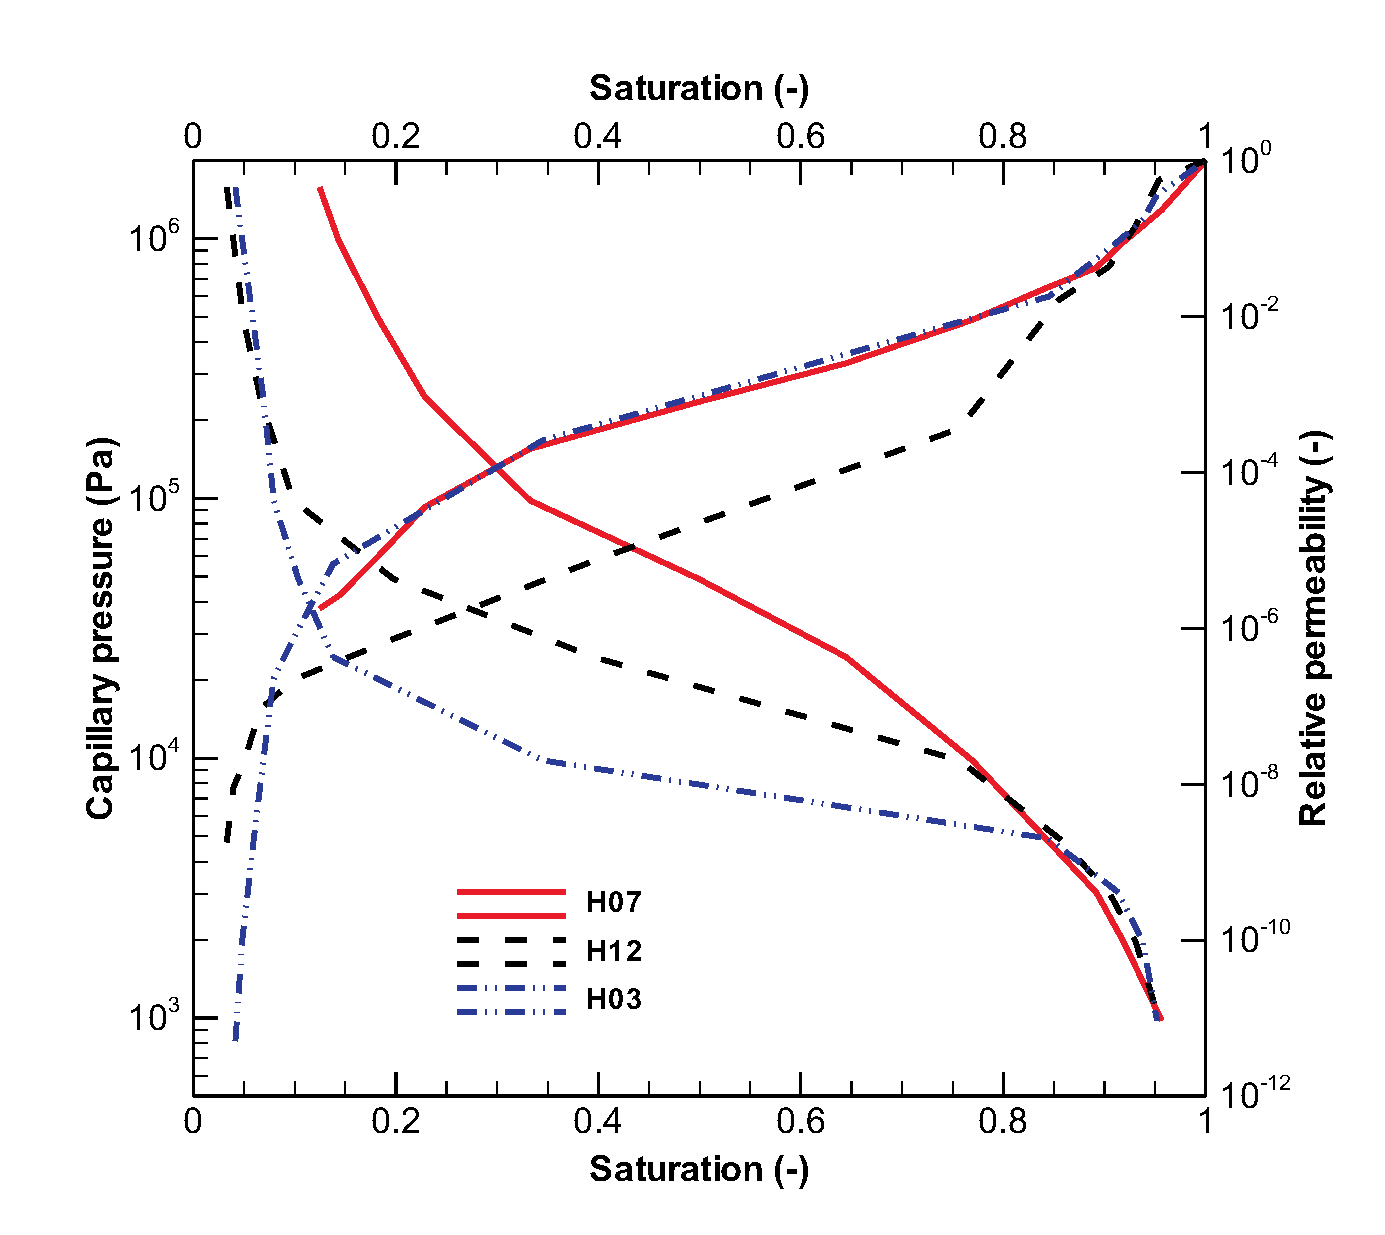
\includegraphics[scale=0.27]{H_US/figures/Soil_P3.eps}
      \end{center}
    \end{minipage}
  %%\hspace{0.01\textwidth}
    \begin{minipage}[t]{0.45\textwidth}
      \begin{center}
        \includegraphics[scale=0.27]{H_US/figures/pl3_s.eps}
      \end{center}
    \end{minipage}\\
  \end{center}
%
  \caption{Soil water characteristic curves (SWCC) (left) and
  time evolution of water saturation in selected soil columns (right)}
  \label{fig:soil_columns}
\end{figure}

\subsubsection*{Benchmark deposit}
\begin{tabular}{|l|l|l|}
  \hline
  Benchmark & Problem type & Path in benchmark deposit \\
  \hline
 \emph{AT\_5} & H & benchmarks\verb \h_us\RSM \\
   \hline
\end{tabular}
